\begin{figure}[htp]
  \centering
  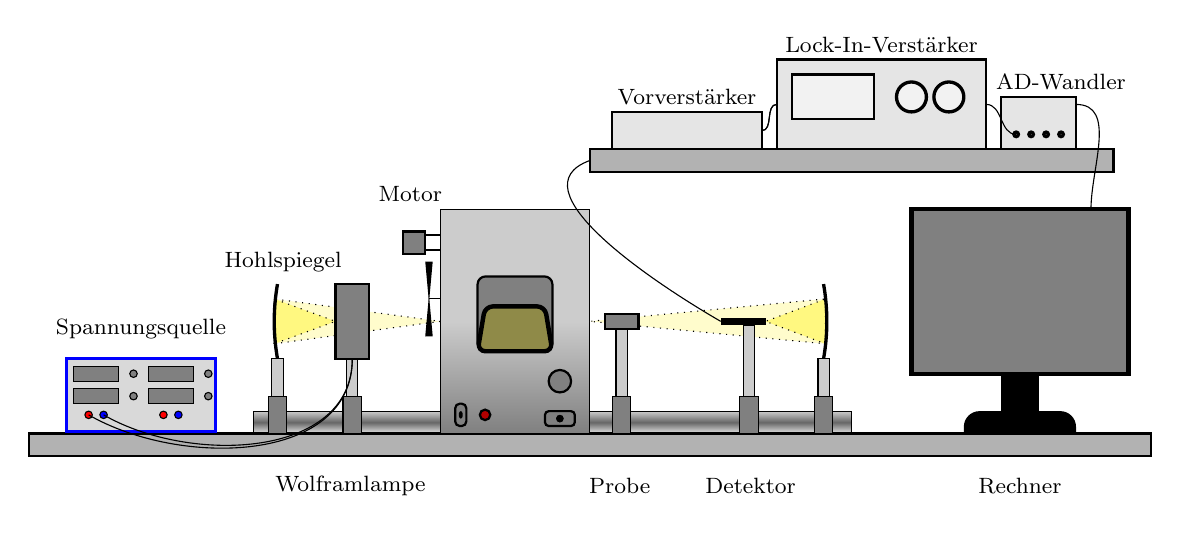
\begin{tikzpicture}[scale=0.95]

    \fill[black, rounded corners = 2mm] (6,-.3)rectangle (7.5,.3);
    \fill[black] (6.5,.3)rectangle (7,.8);
    \filldraw[draw=black, ultra thick, fill=gray] (5.3,.8)rectangle (8.2,3);

    \shadedraw[top color =black!20!white, bottom color=black!10!white, middle color=black!60!white] (-3.5,0) rectangle (4.5,0.3);
    \filldraw[thick, draw = black, fill=black!30!white] (-6.5,0) rectangle (8.5,-.3);
    \shadedraw[top color =black!20!white, bottom color=black!50!white, middle color=black!20!white] (-1,0) rectangle (1,3);
    \filldraw[rounded corners=1mm, thick, fill=gray] (-.5,1.1) rectangle (.5,2.1);
    \filldraw[rounded corners=1mm, ultra thick, fill=yellow!50!black] (-.5,1.1) -- (-.4,1.7) -- (.4,1.7) -- (.5,1.1)-- cycle;
    \filldraw[thick, fill=gray] (.6,.7) circle (.15cm);
    \filldraw[rounded corners=.5mm,thick, fill=gray] (.4,.1) rectangle (.8,.3);
    \fill[black] (.6,.2) circle (.05cm);
    \filldraw[rounded corners=.6mm,thick, fill=gray] (-.8,.1) rectangle (-.65,.4);
    \fill[rounded corners=.3mm,thick, fill=black] (-.75,.2) rectangle (-.7,.3);
    \filldraw[draw=black, thick,fill=red!70!black] (-.4,.25) circle (.07cm);
    \fill[black] (.6,.2) circle (.05cm);
    \filldraw[draw=blue, very thick, fill=black!15!white] (-6,0.025) rectangle (-4,1);
    \filldraw[draw=black, fill = gray] (-5.9,.9) rectangle (-5.3,.7);
    \filldraw[draw=black, fill = gray] (-5.9,.6) rectangle (-5.3,.4);
    \filldraw[draw=black, fill = gray] (-5.1,.8) circle (.05);
    \filldraw[draw=black, fill = gray] (-5.1,.5) circle (.05);
    \filldraw[draw=black, fill = gray] (-4.9,.9) rectangle (-4.3,.7);
    \filldraw[draw=black, fill = gray] (-4.1,.8) circle (.05);
    \filldraw[draw=black, fill = gray] (-4.1,.5) circle (.05);
    \filldraw[draw=black, fill = red] (-5.7,.25) circle (.05);
    \filldraw[draw=black, fill = blue] (-5.5,.25) circle (.05);
    \filldraw[draw=black, fill = red] (-4.7,.25) circle (.05);
    \filldraw[draw=black, fill = blue] (-4.5,.25) circle (.05);
    \filldraw[draw=black, fill = gray] (-4.9,.6) rectangle (-4.3,.4);

    \filldraw[dotted, fill=yellow!20!white](-3.3+0.08,1.2) -- +(0,0.6) -- (-1,1.5) -- cycle;
    \filldraw[dotted, fill=yellow!50!white](-3.3+0.08,1.2) -- +(0,0.6) -- (-2.3-0.1,1.5) -- cycle;
    \filldraw[draw=black, fill=gray] (-3.3,0) rectangle +(0.25,0.5);
    \filldraw[draw=black, fill=black!20!white] (-3.3+0.05,0.5) rectangle +(0.15,0.5);
    \draw[very thick] (-3.3+0.125,1) arc (190:170:3-0.125);

    \filldraw[draw=black, fill=gray] (-2.3,0) rectangle +(0.25,0.5);
    \filldraw[draw=black, fill=black!20!white] (-2.3+0.05,0.5) rectangle +(0.15,0.5);
    \filldraw[thick, fill=gray, draw=black] (-2.3-0.1,1) rectangle +(0.45,1);

    \filldraw[dotted, fill=yellow!20!white](4+0.15,1.2) -- +(0,0.6) -- (1,1.5) -- cycle;
    \filldraw[dotted, fill=yellow!50!white](4+0.15,1.2) -- +(0,0.6) -- (3.35,1.5) -- cycle;

    \filldraw[draw=black, fill=gray] (1.3,0) rectangle +(0.25,0.5);
    \filldraw[draw=black, fill=black!20!white] (1.3+0.05,0.5) rectangle +(0.15,0.9);
    \filldraw[thick, fill=gray, draw=black] (1.3-0.1,1.4) rectangle +(0.45,.2);

    \filldraw[draw=black, fill=gray] (3,0) rectangle +(0.25,0.5);
    \filldraw[draw=black, fill=black!20!white] (3+0.05,0.5) rectangle +(0.15,0.95);
    \fill[thick, fill=black] (3-0.25,1.45) rectangle +(0.6,.1);

    \filldraw[draw=black, fill=gray] (4,0) rectangle +(0.25,0.5);
    \filldraw[draw=black, fill=black!20!white] (4+0.05,0.5) rectangle +(0.15,0.5);
    \draw[very thick] (4+0.125,1) arc (-10:10:3-0.125);

    \filldraw[thick, draw = black, fill=black!30!white] (1,3.5) rectangle (8,3.8);
    \filldraw[thick, draw = black, fill=black!10!white] (1.3,3.8) rectangle (3.3,4.3);
    \filldraw[thick, draw = black, fill=black!10!white] (3.5,3.8) rectangle (6.3,5);
    \filldraw[fill=black!5!white, thick] (3.7,4.2) rectangle (4.8,4.8);
    \filldraw[fill=black!5!white, very thick] (5.8,4.5) circle (.2cm);
    \filldraw[fill=black!5!white, very thick] (5.3,4.5) circle (.2cm);
    \filldraw[thick, draw = black, fill=black!10!white] (6.5,3.8) rectangle (7.5,4.5);
    \filldraw[fill=black!5!white, very thick] (6.7,4) circle (.03cm);
    \filldraw[fill=black!5!white, very thick] (6.9,4) circle (.03cm);
    \filldraw[fill=black!5!white, very thick] (7.1,4) circle (.03cm);
    \filldraw[fill=black!5!white, very thick] (7.3,4) circle (.03cm);

    \filldraw[fill=gray, thick] (-1.5,2.4) rectangle (-1.2,2.7);
    \draw[thick] (-1.2,2.45) -- (-1,2.45);
    \draw[thick] (-1.2,2.65) -- (-1,2.65);
    \draw (-5.5,.25) to[out=-30,in=-90] (-2.3+0.05+0.075,1);
    \draw (-5.7,.25) to[out=-30,in=-90] (-2.3+0.05+0.075,1);

    \fill (-1.2,2.3) -- +(0.1,0) -- (-1.15,1.75) -- cycle;
    \fill (-1.2,1.3) -- +(0.1,0) -- (-1.15,1.85) -- cycle;
    \draw (-1.15, 1.8) -- (-1,1.8);
    \draw (1,3.65) to[out=200,in=150] (3-0.25,1.5);
    \draw (3.3,4.05) to[out=0,in=180] (3.5,4.4);
    \draw (3.3,4.05) to[out=0,in=180] (3.5,4.4);
    \draw (6.3,4.4) to[out=0,in=180] (6.7,4);
    \draw (7.5,4.4) to[out=0,in=90] (7.7,3);

    \node (A) at (1.4,-.7){\footnotesize Probe};
    \node (A) at (3.15,-.7){\footnotesize Detektor};
    \node (A) at (6.75,-.7){\footnotesize Rechner};
    \node (A) at (-2.2,-.7){\footnotesize Wolframlampe};
    \node (A) at (-5,1.4){\footnotesize Spannungsquelle};
    \node (A) at (-3.1,2.3){\footnotesize Hohlspiegel};
    \node (A) at (-1.4,3.2){\footnotesize Motor};
    \node (A) at (7.3,4.7){\footnotesize AD-Wandler};
    \node (A) at (4.9,5.2){\footnotesize Lock-In-Verstärker};
    \node (A) at (2.3,4.5){\footnotesize Vorverstärker};
  \end{tikzpicture}
  \caption{Schematischer Aufbau des SPM2 Prismenspektrographen.}
  \label{fig:ModellSPM2}
\end{figure}
